\documentclass[10pt]{article}

\usepackage[letterpaper,left=0.5in,right=0.5in,top=1in,bottom=1in]{geometry}

\usepackage[T1]{fontenc}
\usepackage[utf8]{inputenc}
\usepackage{lmodern}

\usepackage[activate={true,nocompatibility},final,tracking=true,kerning=true,spacing=true,factor=1100,stretch=10,shrink=10]{microtype}
\microtypecontext{spacing=nonfrench}
\usepackage{xspace}
\usepackage{amssymb,amsfonts,amsmath}
\usepackage{lipsum,xcolor}
\usepackage{graphicx}
\usepackage{float,caption,subcaption,wrapfig}
\usepackage{tcolorbox}
\usepackage{listings}
\usepackage{courier}
\usepackage[english]{babel}
\usepackage{textcomp}
\usepackage{csquotes}
\usepackage{siunitx}
\sisetup{mode=text,
         group-separator={,},
         detect-all,
         binary-units,
         list-units = single,
         range-units = single,
         range-phrase = --,
         per-mode = symbol-or-fraction,
         list-final-separator = {, and }
}

\lstset{basicstyle=\ttfamily,
        breaklines=true,
        numbersep=-8pt,
        numberstyle=\small,
        numbers=right,
        frame = single, 
        showstringspaces=false,    
        keywordstyle=\color{blue}\bf,
        commentstyle=\color{darkgray},
        stringstyle=\color{purple}\bf,
  }

\DeclareSIUnit\atm{atm}
\DeclareSIUnit\bar{bar}

\headheight = 13.6pt
\usepackage{fancyhdr}
\pagestyle{fancy}

\lhead{PH 641 Sp2020}
\chead{Assignment 1}
\rhead{Due 11:59 pm, 17 March 2020}

\rfoot{Submitted by: Paige Lorson}
\tcbset{width=(\linewidth-2mm),before=,after=\hfill,colframe=black,colback=white,}
\newcommand{\volume}{{\ooalign{\hfil$V$\hfil\cr\kern0.08em--\hfil\cr}}}
\newenvironment{Solution}
    {\textbf{Solution:}
    
    \vspace{5mm}
    \begin{tcolorbox}
    }
    {
    \end{tcolorbox}
    \vspace{5mm}
    % \newpage
    }
\newcommand{\vol}{{\ooalign{\hfil$V$\hfil\cr\kern0.08em--\hfil\cr}}}
\renewcommand\labelitemi{$\cdot$}

\begin{document}

% \noindent\textbf{Note:} This survey serves to inform your instructor and to test the homework submission via gradescope. It will be graded like a regular homework set.

\begin{enumerate}

%%%%%%%%%%%%%%%%%%%%%%%%%%%%%%%%%%%%%%%%%%%%%%%


\item The function  $U$ is given by $U\left(S,\vol,N\right) = {\left(S^2+S-\vol^2\right)}/{N}$. Give three reasons why this is not a correct function describing the internal energy of a material.


\begin{Solution}
\begin{enumerate}
    \item The units of problem could not work out as written. You can't add entropy with entropy squared.
    \item From the TD equation, the partial derivative of $U$ with respects to $S$ is $T$. That is not the case for this expression.
    \item From the TD equation, the partial derivative of $U$ with respects to $\vol$ is $-p$. That is not the case for this expression.

\end{enumerate}
\end{Solution}
\newpage

\item The internal energy of a system is given by  $U\left(S,\vol,N\right) = {\left(S^\alpha \vol^\beta N^\gamma \right)}$
\begin{enumerate}
    \item Using the fact that $U$ is extensive, find a relation between $\alpha$, $\beta$, and $\gamma$.
    
    \begin{Solution}
    For U extensive, we can say,
    \begin{equation}\label{extensive}
    U(S, \vol, N)=\frac{\partial U(S, \vol, N)}{\partial S} S + \frac{\partial U(S, \vol, N)}{\partial \vol} \vol + \frac{\partial U(S, \vol, N)}{\partial N} N
    \end{equation}
    This means,
    
    \begin{align}
    \frac{\partial U(S, \vol, N)}{\partial S}  &=  \alpha S^{\alpha-1} \vol^\beta N^\gamma \\
    \frac{\partial U(S, \vol, N)}{\partial \vol} &=  \beta S^{\alpha} \vol^{\beta-1} N^\gamma \\
    \frac{\partial U(S, \vol, N)}{\partial N} &= \gamma S^{\alpha} \vol^{\beta} N^{\gamma-1}
    \end{align}
    Substituting these back into \ref{extensive} we get,
    \begin{align}
    U(S, \vol, N)&= \alpha S^\alpha \vol^\beta N^\gamma  + \beta S^\alpha \vol^\beta N^\gamma  + \gamma S^\alpha \vol^\beta N^\gamma \\
    &=\left(\alpha + \beta + \gamma\right) S^\alpha \vol^\beta N^\gamma 
    \end{align}
    Form the problem statement, we know that $U \left(S,\vol,N\right) = {\left(S^\alpha \vol^\beta N^\gamma \right)}$ so,
    \begin{equation}
        \boxed{
        \left(\alpha + \beta + \gamma\right) = 1
        }
    \end{equation}
    \end{Solution}
    % \newpage 
    \item Calculate the pressure $p$, temperature 
    $T$, and chemical potential $\mu$ as a function of $S$, $\vol$, and $N$.
    
    \begin{Solution}
    From the TD Equation, recall, 
    \begin{equation}
        dU = T dS - p d\vol + \mu dN
    \end{equation}
    where, 
    \begin{equation}
        \left.\frac{\partial U}{\partial S}\right|_{\scriptsize{\vol}, N} = T \qquad \left.\frac{\partial U}{\partial \vol}\right|_{S, N} = -p \qquad \left.\frac{\partial U}{\partial N}\right|_{\scriptsize{S,\vol}} = \mu  
    \end{equation}
    From the previous part, this means, 
    \begin{equation}
        \boxed{
        T\left(S, \vol, N\right) = \alpha S^{\alpha-1} \vol^\beta N^\gamma
        }
    \end{equation}
    \begin{equation}
        \boxed{
        p\left(S, \vol, N\right) = -\beta S^{\alpha} \vol^{\beta-1} N^\gamma
        }
    \end{equation}
    \begin{equation}
        \boxed{
        \mu\left(S, \vol, N\right) = \gamma S^{\alpha} \vol^{\beta} N^{\gamma-1}
        }
    \end{equation}
    
    \end{Solution}
    \newpage 


    \item Calculate the heat capacity at constant volume $\vol$(and constant $N$).
    
    \begin{Solution}    
    The Constant volume heat capacity is the partial derivative of $U$ with respects to $T$. So,
    
    \begin{equation}
        C_v = \left.\frac{\partial U}{\partial T}\right|_{\scriptsize{\vol},N} = T\left.\frac{\partial S}{\partial T}\right|_{\scriptsize{\vol},N}
    \end{equation}


    We can use the previous parts and the Euler equation for extensive systems to get an expression for $U$ in terms of $T$.
    
    \begin{align}
        U &= TS - p\vol + \mu N\\
        &= T S + \beta S^\alpha \vol^\beta N^\gamma + \gamma S^\alpha \vol^\beta N^\gamma
    \end{align}
    The total derivative of this, with $N$ and $\vol$ both constant,
    \begin{align}
        dU &= \left.\frac{\partial U}{\partial T}\right|_S dT + \left.\frac{\partial U}{\partial S}\right|_T dS\\
        &= S dT + \left[T + \beta\alpha S^{\alpha-1}\vol^\beta N^\gamma + \gamma\alpha S^{\alpha-1}\vol^\beta N^\gamma\right]dS
    \end{align}
    
    That makes the constant volume heat capacity
    \begin{equation}
    \boxed{
    C_v = S
    }        
    \end{equation}
    However... this seems incorrect... 
    An alternate approach: 
        \begin{equation}
        % \left.\frac{\partial S}{\partial T}\right|_{\scriptsize{\vol},N} = \left[\frac{\partial U}{\partial S}\right]_{\scriptsize{\vol}, N}^{-1} \left.\frac{\partial U}{\partial T}\right|_{\scriptsize{\vol},N}
        \left.\frac{\partial S}{\partial T}\right|_{\scriptsize{\vol},N} = \left.\frac{\partial \left[ \frac{T^{1/\alpha}}{\left[\alpha \scriptsize{\vol}^{\beta}N^{\gamma} \right]^{1/\alpha}} \right]}{\partial T}\right|_{\scriptsize{\vol},N} = \frac{1}{\alpha}\left[ T^{1/\alpha-1}\left[\alpha \scriptsize{\vol}^{\beta}N^{\gamma} \right]^{-1/\alpha} \right]
    \end{equation}
    \begin{equation}
    \boxed{
        C_v = \frac{1}{\alpha}\left[\frac{T}{\alpha \scriptsize{\vol}^{\beta}N^{\gamma}} \right]^{-1/\alpha}
        }
    \end{equation}
    
    \end{Solution}
    \newpage 

    \item Calculate the adiabatic compressibility (at constant $N$).
    
    \begin{Solution}    
    The adiabatic compressibility is given as,
    \begin{equation}
        \kappa_S = -\frac{1}{\vol}\left.\frac{\partial \vol}{\partial p}\right|_{S, N}
    \end{equation}
    The partial, $\left.\partial \vol/\partial p\right|_{S, N}$ is equivalent to $\left[\partial p/\partial \vol\right]_{S, N}^{-1}$, so
    \begin{equation}
        \left.\frac{\partial \vol}{\partial p}\right|_{S, N} = \left[-\beta\left(\beta-1\right) S^{\alpha} \vol^{\beta-2} N^\gamma \right]^{-1}
    \end{equation}
    Thus,
    \begin{align}
        \kappa_S &= -\frac{1}{\vol}\left.\frac{\partial \vol}{\partial p}\right|_{S, N} = -\frac{1}{\vol \left[-\beta\left(\beta-1\right) S^{\alpha} \vol^{\beta-2} N^\gamma \right]}\\
        &= \frac{-1}{-\beta\left(\beta-1\right)S^{\alpha} \vol^{\beta-1} N^\gamma}\\
        &\boxed{=\frac{-1}{p\left(\beta-1\right)}
        }
    \end{align}
    \end{Solution}
    % \newpage 
    
    \item Based on the sign of these response functions (assume $C_v \geq 0$, $\kappa_s \geq 0$, we will prove this later), find inequalities for $\alpha$ and $\beta$.
    
    \begin{Solution}    
    If $\kappa_s \geq 0$, then \boxed{\beta<1}. If $C_v \geq 0$, then \boxed{\alpha>0}. 
    
    \end{Solution}
\newpage 

\end{enumerate}

\item Given the equations below ($N$, $\kappa_B$, $a$, and $b$ are constants):

\begin{equation}
    p = \frac{N\kappa_B T}{\vol -b N}-\frac{a N^2}{\vol^2} \qquad U = \frac{3}{2} N \kappa_B T - \frac{a N^2}{\vol}
\end{equation}

Evaluate the requested partial derivative: 

\begin{enumerate}
    \item $\left.\frac{\partial p}{\partial \scriptsize{\vol}}\right|_T$
    
    
    \begin{Solution}
    Since $N$, $\kappa_B$, $a$, and $b$ are constants, $p = p\left(\vol, T\right)$. To get the partial derivative $\left.\frac{\partial p}{\partial \vol}\right|_T$, we can allow $\vol$ to vary while holding $T$ constant.
    
    \begin{equation}
    \boxed{
        \left.\frac{\partial p}{\partial \vol}\right|_T =  \frac{a N^2}{\vol^3} - \frac{N\kappa_B T}{\left(\vol -b N\right)^2}
    }
    \end{equation}
    
    \end{Solution}
    % \newpage 

    \item $\left.\frac{\partial U}{\partial \scriptsize{\vol}}\right|_p$
    

    \begin{Solution}
    $U$ is a function of $T$ and $\vol$. We can use the expression for $p$ to get $U$ as a function of $T$ and $p$. 
    
    \begin{equation}
        T = \frac{\vol}{N\kappa_B} -\frac{b N p}{N\kappa_B} +  \frac{a N}{\vol\kappa_B} - \frac{a b N^2}{\vol^2\kappa_B}
    \end{equation}
    \begin{align}
        U\left(\vol, p\right) &= \frac{3}{2} N \kappa_B \left[\frac{\vol}{N\kappa_B} -\frac{b N p}{N\kappa_B} + \frac{a N}{\vol\kappa_B} - \frac{a b N^2}{\vol^2\kappa_B}\right] - \frac{a N^2}{\vol}
        \\
        &= \frac{3\vol}{2} - \frac{3 b N p}{2} + \frac{ a N^2}{2 \vol} - \frac{3 a b N^3}{2 \vol^2} 
    \end{align}

    Now, the partial derivative of $U$ with respect to $\vol$, holding $p$ constant is 
    
    \begin{equation}
       \boxed{
       \left.\frac{\partial U}{\partial \vol}\right|_p = \frac{3}{2} - \frac{ a N^2}{2 \vol^2} + \frac{3 a b N^3}{ \vol^3}
       }
    \end{equation}

    \end{Solution}

\end{enumerate}
\newpage 

\item In traditional thermodynamics, one defines the pressure as minus the change in energy with volume $P = -\left.{ \partial E /\partial\vol  }\right|_{N,S}$, and the chemical potential as the change in energy with number of particles $\mu = \left.\partial E/\partial N \right|_{\scriptsize{\vol}, S}$. The total internal energy satisfies
\begin{equation}\label{p4-1}
    dE = T d S - P d\vol +\mu dN
\end{equation}
\begin{enumerate}
    \item \label{3.10a} Show by solving equation \ref{p4-1} for $dS$ that $ \left.\partial S/\partial \vol \right|_{N, E} = P/T$ and $ \left.\partial S/\partial N \right|_{\scriptsize{\vol}, E} = -\mu/T$. I have always been uncomfortable with manipulating $dX$s. How can we derive these relations with traditional partial derivatives? Our equation of state $S\left(E, \vol, N \right)$ at fixed $N$ is a surface embedded in three dimensions. EOPC Figure 3.4 shows a triangle on this surface, which we can use to derive a general triple-product relation between partial derivatives.
    
    
    \begin{Solution}

    Solving for $dS$ we get
    \begin{equation}
     dS = \frac{dE}{T} + \frac{p d\vol}{T} -\frac{\mu dN}{T} 
    \end{equation}
    The total derivative of $S(E,\vol,N)$ will have the form,
    \begin{equation}
         dS = \left.\frac{\partial S}{\partial E} \right|_{N, \scriptsize{\vol}}  dE + \left.\frac{\partial S}{\partial N} \right|_{\scriptsize{\vol}, E} dN + \left.\frac{\partial S}{\partial \vol} \right|_{N, E} d\vol
    \end{equation}
    This means, 
    \begin{equation}
    \boxed{
         \left.\frac{\partial S}{\partial E} \right|_{N, \scriptsize{\vol}} = \frac{1}{T} 
         \qquad  \left.\frac{\partial S}{\partial N} \right|_{\scriptsize{\vol}, E} = -\frac{\mu}{T}
         \qquad  \left.\frac{\partial S}{\partial \vol} \right|_{N, E} = \frac{P}{T}
         }
    \end{equation}
    \end{Solution}
    \newpage 
    
    \item \label{3.10b} Show, if $f$ is a function of $x$ and $y$ that 
    \begin{equation}
        \left.\frac{\partial x}{\partial y}\right|_f 
        \left.\frac{\partial y}{\partial f}\right|_x 
        \left.\frac{\partial f}{\partial x}\right|_y = -1
    \end{equation}
    (Hint:  Consider the triangular path in EOPC Fig. 3.4. The first side starts at $(x_0 , y_0 , f_0 )$ and moves along a contour at constant $f$ to $y_0+\Delta y$. The resulting vertex will thus be at $\left(x_0+\left. {\partial x/\partial y}\right|_f \Delta y, y_0+\Delta y, f_0\right)$. The second side runs at constant $x$ back to $y_0$, and the third side runs at constant y back to $(x_0 , y_0 , f_0 )$. The curve must close to make $f$ a single-valued function; the resulting equation should imply the triple-product relation.)
    
    \begin{Solution}
    If $f = f(x,y)$ then,
    \begin{align}
        d f&=\left.\frac{\partial f}{\partial x}\right|_{y} d x+\left.\frac{\partial f}{\partial y}\right|_{x} d y\\
        d x&=\left.\frac{\partial x}{\partial f}\right|_{y} d f+\left.\frac{\partial x}{\partial y}\right|_{f} d y\\
        d y&=\left.\frac{\partial y}{\partial f}\right|_{x} d f+\left.\frac{\partial y}{\partial x}\right|_{f} d x
    \end{align}
    We next can substitute one of expressions into one of the others and compare coefficients. This gets us,
    \begin{equation}
        d x=\left.\frac{\partial x}{\partial f}\right|_{y} d f+\left.\frac{\partial x}{\partial y}\right|_{f}\left[\left.\frac{\partial y}{\partial f}\right|_{x} d f+\left.\frac{\partial y}{\partial x}\right|_{f} d x\right]
    \end{equation}
    For $d f$,
    \begin{equation}
        0 = \left.\frac{\partial x}{\partial f}\right|_{y} + \left.\frac{\partial x}{\partial y}\right|_{f}\left.\frac{\partial y}{\partial f}\right|_{x}
    \end{equation}
    and for $d x$,
    \begin{equation}
        1 = \left.\frac{\partial y}{\partial x}\right|_{f} \left.\frac{\partial x}{\partial y}\right|_{f}
    \end{equation}
    We can combine these two expressions to get,
    \begin{equation}
    \boxed{
        \left.\frac{\partial x}{\partial y}\right|_f \left.\frac{\partial y}{\partial f}\right|_x \left.\frac{\partial f}{\partial x}\right|_y = -1
        }
    \end{equation}
    \end{Solution}
    \newpage 
    \item Starting from the ‘traditional’ definitions for $P$ and $\mu$, apply your formula from part \ref{3.10b} to $S$ at fixed $E$ to derive the two equations in part \ref{3.10a} again. (This last calculation is done in the reverse direction in EOPC Section 3.4.)
    
    \begin{Solution}
    
    Given $S = S(E,\vol,N)$ and fixing $N$, then, we can say
    \begin{align}
        \left.\frac{\partial \vol}{\partial E}\right|_{S,N} \left.\frac{\partial E}{\partial S}\right|_{\scriptsize{\vol},N} \left.\frac{\partial S}{\partial \vol}\right|_{E,N} &= -1\\
        &= \frac{P}{T}\left(1 /\left.\frac{\partial E}{\partial \vol}\right|_{S, N}\right) T
    \end{align}
    thus,
    \begin{equation}
        \boxed{
        \left.\frac{\partial E}{\partial \vol}\right|_{S, N} = -P
        }
    \end{equation}
    Now by fixing $\vol$,
    \begin{align}
        \left.\frac{\partial N}{\partial E}\right|_{S, \scriptsize{\vol}} \left.\frac{\partial S}{\partial N}\right|_{E, \scriptsize{\vol}} \left.\frac{\partial E}{\partial S}\right|_{N, \scriptsize{\vol}} &= -1\\
        &= -\frac{\mu}{T}\left(1 /\left.\frac{\partial E}{\partial N}\right|_{S, \scriptsize{\vol}}\right) T
    \end{align}
    thus,
    \begin{equation}
        \boxed{
        \left.\frac{\partial E}{\partial N}\right|_{S, \scriptsize{\vol}} = \mu
        }
    \end{equation}
        
    \end{Solution}
\end{enumerate}
\newpage 

\item A monatomic ideal gas in a piston is cycled around the path in the $P -\vol$ diagram in Fig. 5.15. Leg $a$ cools at constant volume by connecting to a heat bath at $T_c$; leg $b$ heats at constant pressure by connecting to a heat bath at $T_h$ ; leg $c$ compresses at constant temperature while remaining connected to the bath at $T_h$.
Which of the following six statements are true?
\begin{enumerate}
    \item \textbf{(T)} The cycle is reversible; no net entropy is created in the Universe.
    
    \item \textbf{(T)} The cycle acts as a refrigerator, using work from the piston to draw energy from the cold bath into the hot bath, cooling the cold bath.
    
    
    \item \textbf{(F)} The cycle acts as an engine, transferring heat from the hot bath to the cold bath and doing positive net work on the outside world.
    
    
    \item \textbf{(F)} The work done per cycle has magnitude $\left|W\right| = P_0 \vol_0 \left|4 \log{4} - 3\right|$.
    
    
    \item \textbf{(T)} The heat transferred into the cold bath, $Q_c$ , has magnitude $\left|Q_c \right| = \left(9/2\right)P_0 \vol_0$.
    
    \item \textbf{(T)} The heat transferred from the hot bath, $Q_h$ , plus the net work $W$ done by the piston onto the gas, equals the heat $Q_c$ transferred into the cold bath.
    
    
\end{enumerate}

\newpage

\item A thermodynamic system consists of two identical subsystems, $\alpha=\{1,2\}$ described by thermodynamic variables $T_{a}, U_{a}=C\left(T_{a}-T_{0}\right)+U_{0},$ and $S_{a}\left(T_{a}\right)$

\begin{enumerate}

\item Determine $S_{a}\left(T_{a}\right)$ for the individual subsystems.

\begin{Solution}
Recall from the TD equation that for a constant $\vol$ and $N$,
\begin{equation}\label{dutds}
    dU = T dS
\end{equation}
We also know from the problem statement that $dU = CdT$. We can equate these two statements and integrate both sides from $S_0, T_0$ to $S_a, T_a$ to get the following expression for $S_a$ (Note: The reference state for $S_a$ is set to the initial temperature such that $S_0 = 0$).
\begin{equation}
\boxed{
    S_a = C \ln{\frac{T_a}{T_0}}
    }
\end{equation}

\end{Solution}
% \newpage

\item Determine $U\left(T_{1}, T_{2}\right)$ and $S\left(T_{1}, T_{2}\right)$ for the total system.
Now, consider the total system, where the two subsystems can exchange energy with each other but not with any external environment. The initial energies and initial temperatures of the two subsystems are $U_{0, 1}$ and $U_{0, 2}$ and $T_{0, 1}$ and $T_{0, 2}$ respectively.

\begin{Solution}
% Because $U$ and $S$ are both extensive, the values for the entire system will be double that of the identical individual systems.
\begin{equation}
    \boxed{
    U_{a} = C \left(T_{a,1}-T_{0,1}\right)+U_{0,1} + C \left(T_{a,2}-T_{0,2}\right)+U_{0,2}
    }
\end{equation}
\begin{equation}
\boxed{
    S_a = C \ln{\frac{T_{a,1}}{T_{0,1}}} + C \ln{\frac{T_{a,2}}{T_{0,2}}}
    } = \boxed{
    C \ln{\frac{T_{a,1}T_{a,2}}{T_{0,1}T_{0,2}}}}
\end{equation}
\end{Solution}
\newpage

\item Determine and plot the entropy of the total system and discuss it as a function of $U_{1}$. (For the graph of $S\left(U_{1}\right)$ use $U_{0, 1}=3 C T_{0}$ and $U_{0, 2}=C T_{0}$.)

\begin{Solution}

We can get the temperature of each system as a function of $U$,
\begin{equation}
    T_{a,\alpha} = \frac{U_{a,\alpha} - U_{0,\alpha}}{C}+T_{0,\alpha}
\end{equation}
We can use this with the definitions for $U_{0,\alpha}$ to get $S_a(U)$

\begin{equation}
    S_a =  C \ln{\frac{\left(\frac{U_{a,1}}{C} - 2 T_{0,1} \right) \left(\frac{U_{a,2}}{C}\right)}{T_{0,1}T_{0,2}}} 
\end{equation}
Now recall that $U = U_1 + U_2$,  so 
\begin{align}
    S_a &=  C \ln{\frac{\left(\frac{U_{a,1}}{C} - 2 T_{0,1} \right) \left(\frac{U_a - U_{a,1} }{C}\right)}{T_{0,1}T_{0,2}}}\\
    &\boxed{= C \ln{\frac{U_{a}U_{a,1} + 2CT_{0,1}U_{a,1} - U_{a,1}^2 - 2CT_{0,1}U_{a}}{C^2 T_{0,1}T_{0,2}}}}
\end{align}
The total internal energy is conserved, so it is a constant. The initial temperatures and $C$ are also constant. Thus, $S$ is only a function of $U_1$ and has the form,
\begin{equation}
    S_a = C \ln{a U_{a,1} - b U_{a,1}^2 + c}
\end{equation}

This function will have the form, 

\centering{
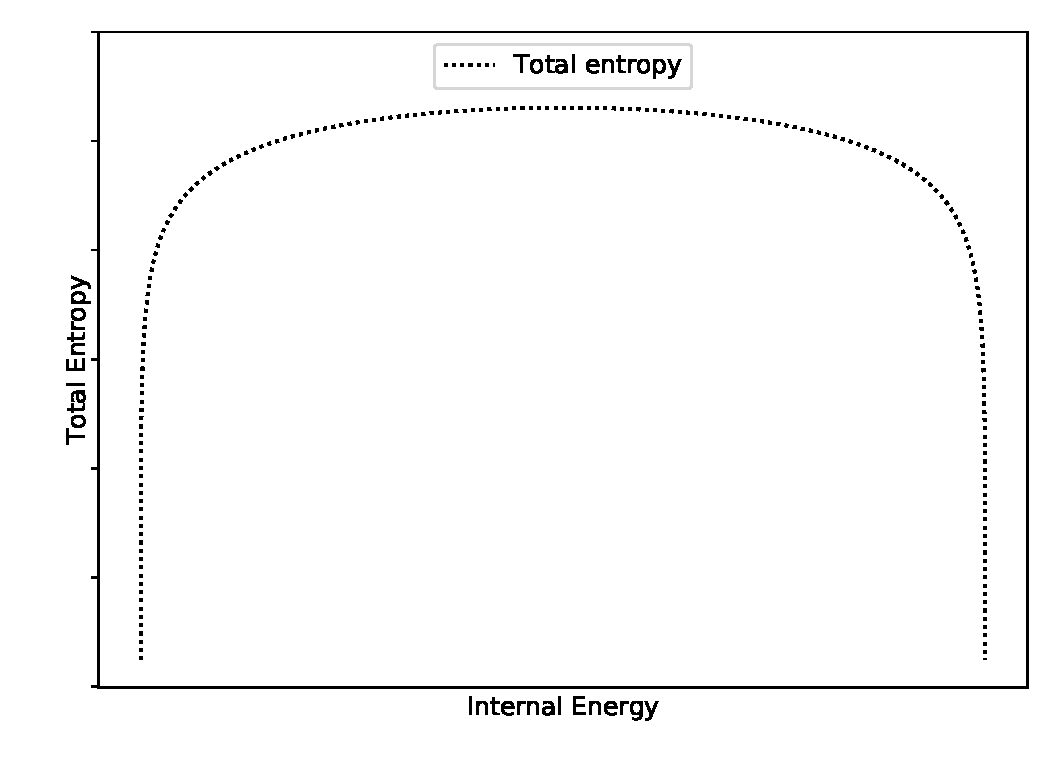
\includegraphics[width=4in]{Assignments/plot_a1.pdf}}
\end{Solution}
\newpage

\item Using the maximum principle for the entropy, determine the equilibrium temperatures and energies for the two subsystems.

\begin{Solution}
The entropy will be maximized at the temperature for which $d S = 0$. 
 
So,

\begin{align}
    d S &= \frac{\partial S}{\partial T_{a,1}}d T_{a,1} + \frac{\partial S}{\partial T_{a,2}}d T_{a,2} = 0\\
    &=C\left[ \frac{T_{0,1}T_{0,2}}{T_{a,1}T_{a,2}} \right]\left[ \frac{T_{a,2}}{T_{0,1}T_{0,2}} \right]d T_{a,1} + C \left[ \frac{T_{0,1}T_{0,2}}{T_{a,1}T_{a,2}} \right]\left[ \frac{T_{a,1}}{T_{0,1}T_{0,2}} \right]d T_{a,2} = 0\\
    &= \frac{1}{T_{a,1}} d T_{a,1} + \frac{1}{T_{a,2}} d T_{a,2} = 0 
\end{align}
This means entropy is maximized when,
\begin{equation}
    \ln{T_{a,1}} = \ln{T_{a,1}}
\end{equation}
\begin{equation}
   \boxed{ T_{a,1}=T_{a,2}}
\end{equation}

\end{Solution}
% \newpage

\item Determine the entropy increase for the total system after reaching equilibrium as a function of $T_{0, 1}$ and $T_{0, 2}$

\begin{Solution}
The total entropy at equilibrium will be,

\begin{equation}
    S_a = C \ln{\frac{T_{a}^2}{T_{0,1}T_{0,2}}}
\end{equation}
\end{Solution}
\newpage

\item Now consider the case where $T_{0, 1}$ and $T_{0, 2}$ differ only slightly from the equilibrium temperature $T_{f}$ of the total system: $T_{0, 1}=T_{f}+\Delta T / 2$ and $T_{0, 2}=$ $T_{f}-\Delta T / 2 .$ Determine the entropy gain $\Delta S=S_{f}-S_{0}$ up to second order in $\Delta T$ and $\mathrm{up}$ to first order in $\Delta T$ for the individual subsystems. Interpret the result.

\begin{Solution}
The change in entropy can be expressed as,
\begin{equation}
    dS = \frac{C}{T_1}d T_1 + \frac{C}{T_2}d T_2 
\end{equation}
For second order accuracy,
\begin{equation}
    S_f = S\left(T_{0,1}, T_{0,2}\right) + \left[ \frac{\partial S}{\partial T_1} \Delta T +  \frac{\partial S}{\partial T_2} \Delta T\right] + \frac{1}{4}\left[ \frac{\partial^2 S}{{\partial T_1}^2} {\Delta T}^2 + \frac{\partial^2 S}{{\partial T_2}^2} {\Delta T}^2\right]
\end{equation}
where,
\begin{align}
    \frac{\partial S}{\partial T_1} = \frac{C}{T_{0,1}} \qquad& \qquad \frac{\partial S}{\partial T_2} = \frac{C}{T_{0,2}}\\
    \frac{\partial^2 S}{{\partial T_1}^2} = -\frac{C}{T_{0,1}^2} \quad & \quad \frac{\partial^2 S}{{\partial T_2}^2} = -\frac{C}{T_{0,2}^2}
\end{align}
So, 
\begin{equation}
    S_f = S\left(T_{0,1}, T_{0,2}\right) + \left[ \frac{C}{T_{0,1}} \Delta T +  \frac{C}{T_{0,2}} \Delta T\right] - \frac{1}{4}\left[ \frac{C}{T_{0,1}^2} {\Delta T}^2 +\frac{C}{T_{0,2}^2} {\Delta T}^2\right]
\end{equation}
This can be simplified to 
\begin{equation}
    S_f = S\left(T_{0,1}, T_{0,2}\right) + C\Delta T\left[ \frac{1}{T_{0,1}} +  \frac{1}{T_{0,2}} \right] - \frac{C{\Delta T}^2}{4}\left[ \frac{1}{T_{0,1}^2} + \frac{1}{T_{0,2}^2}\right]
\end{equation}
Since the first order term will be larger than the second order term and the first order term is strictly positive, the small change will cause an increase in $S$, as expected.
\end{Solution}
% \newpage

\item Express the entropy $S\left(U_{f}\right)$ and energy $U\left(T_{f}\right)$ of the total system after reaching equilibrium in terms of the total energy $U_{f}$ and equilibrium temperature $T_{f} .$ Discuss your result.

\begin{Solution}
\begin{equation}
    U_f = 2C T_f + 3C T_{0,1} + C T_{0,2}
\end{equation}
\begin{equation}
    T_f = \frac{1}{2C}U_f - \frac{3}{2} T_{0,1} - \frac{1}{2} T_{0,2}
\end{equation}
\begin{equation}
    S_a = C \ln{\frac{\left(\frac{1}{C}U_f - 3 T_{0,1} -  T_{0,2}\right)^2}{4T_{0,1}T_{0,2}}}
\end{equation}
These results are consistant with previous parts.
\end{Solution}
% \newpage
    
\end{enumerate}
\end{enumerate}
\end{document}
